%%%%%%%%%%%%%%%%%%%%%%%%%
%% Header for standard beamer presentation
%%
%%  PresentationHeader.tex
%%
%%%%%%%%%%%%%%%%%%%%%%%%%

\documentclass[english,10pt]{beamer}

%%%%%%%%%%%%%%%%%%%%
%% Include general header where common packages are defined
%%%%%%%%%%%%%%%%%%%%

% general packages without options
\usepackage{amsmath,amssymb,bbm}




%%%%%%%%%%%%%%%%%%%%
%% Idem general commands
%%%%%%%%%%%%%%%%%%%%

%%% Commands

\newcommand{\noun}[1]{\textsc{#1}}


%% Math

% Operators
\DeclareMathOperator{\Cov}{Cov}
\DeclareMathOperator{\Var}{Var}
\DeclareMathOperator{\E}{\mathbb{E}}
\DeclareMathOperator{\Proba}{\mathbb{P}}

\newcommand{\Covb}[2]{\ensuremath{\Cov\!\left[#1,#2\right]}}
\newcommand{\Eb}[1]{\ensuremath{\E\!\left[#1\right]}}
\newcommand{\Pb}[1]{\ensuremath{\Proba\!\left[#1\right]}}
\newcommand{\Varb}[1]{\ensuremath{\Var\!\left[#1\right]}}

% norm
\newcommand{\norm}[1]{\| #1 \|}


% amsthm environments
\newtheorem{definition}{Definition}



%% graphics

% renew graphics command for relative path providment only ?
%\renewcommand{\includegraphics[]{}}






\usetheme{Warsaw}

\setbeamertemplate{footline}[text line]{}
\setbeamercolor{structure}{fg=purple!50!blue, bg=purple!50!blue}

\setbeamercovered{transparent}


% shortened command for a justified frame
\newcommand{\jframe}[2]{\frame{\frametitle{#1}\justify{#2}}}



%%%%%%%%%%%%%%%%%%%%%
%% Begin doc
%%%%%%%%%%%%%%%%%%%%%

\begin{document}



\title{Thesis Progress Meeting}


\author{J.~Raimbault$^{1,2}$}

\institute{$^{1}$G{\'e}ographie-cit{\'e}s (UMR 8504 CNRS)\\
$^{2}$LVMT (UMR-T 9403 IFSTTAR)}


\date{May 3rd 2016}


%%%%%%%%%%%%%%%%%%%%%%%%%%%%%%%%
\begin{frame}
\titlepage
\end{frame}

%\begin{frame}
%\tableofcontents
%\end{frame}
%%%%%%%%%%%%%%%%%%%%%%%%%%%%%%%%



\section{Achieved Work}


\jframe{Achieved Work (by projects)}{
\begin{itemize}
\item Network Necessity [1.2w]
\item Density Generation (paper and toy-models tests) [0.4w]
\item Biblio/Meetings/Organisation [1.2w] ; Reading Records [0.3w]
\item Cybergeo Project [1w] (ETA 1w)
\item Side projects (Discrepancy, Transportation Equilibrium, Ecology) [4w] (ETA 3w)
\end{itemize}
}



\section{Network Necessity}

\sframe{Network Necessity}{
\textbf{Simple toy models to test theoretical assumption of network necessity}

\medskip

$\rightarrow$ Extended Gibrat model for population growth within a city system (simplified Favaro-Pumain model or projected Cottineau-1.y.z model) with interactions. \textit{Idea :} Test if physical Network (feedback of physical flows) allows a better fit.

\medskip

\textbf{Rq. :} a lot of confusion on Gibrat Model :
\begin{enumerate}
\item Under classical independence assumptions, $Law(P)$ is known at any $t$ whatever the distribution of growth rates : no need to simulate).
\item Furthermore, various formulation are possible : independent realizations across cities of the same random process $P(t)$ with varying non-stationary parameters $\mu(t)$, with interdependence captured in recurrence relation between successive expectancies ; or multi-dimensional random process $(P_i(t))$ with covariance structure $\Covb{P_i}{P_j}$ estimated in time.
\end{enumerate}

}

\sframe{Empirical Results}{

\textit{Work on Pumain-INED French cities database.}

\medskip

\textbf{Growth Rates are more log-normal than normal ! } (simple likelihood tests) - in fact $\Delta \log P$ closer from levy fat-tail distribution.

\medskip

\textbf{Non-stationarity of correlations in time and space : }

\smallskip

\centering
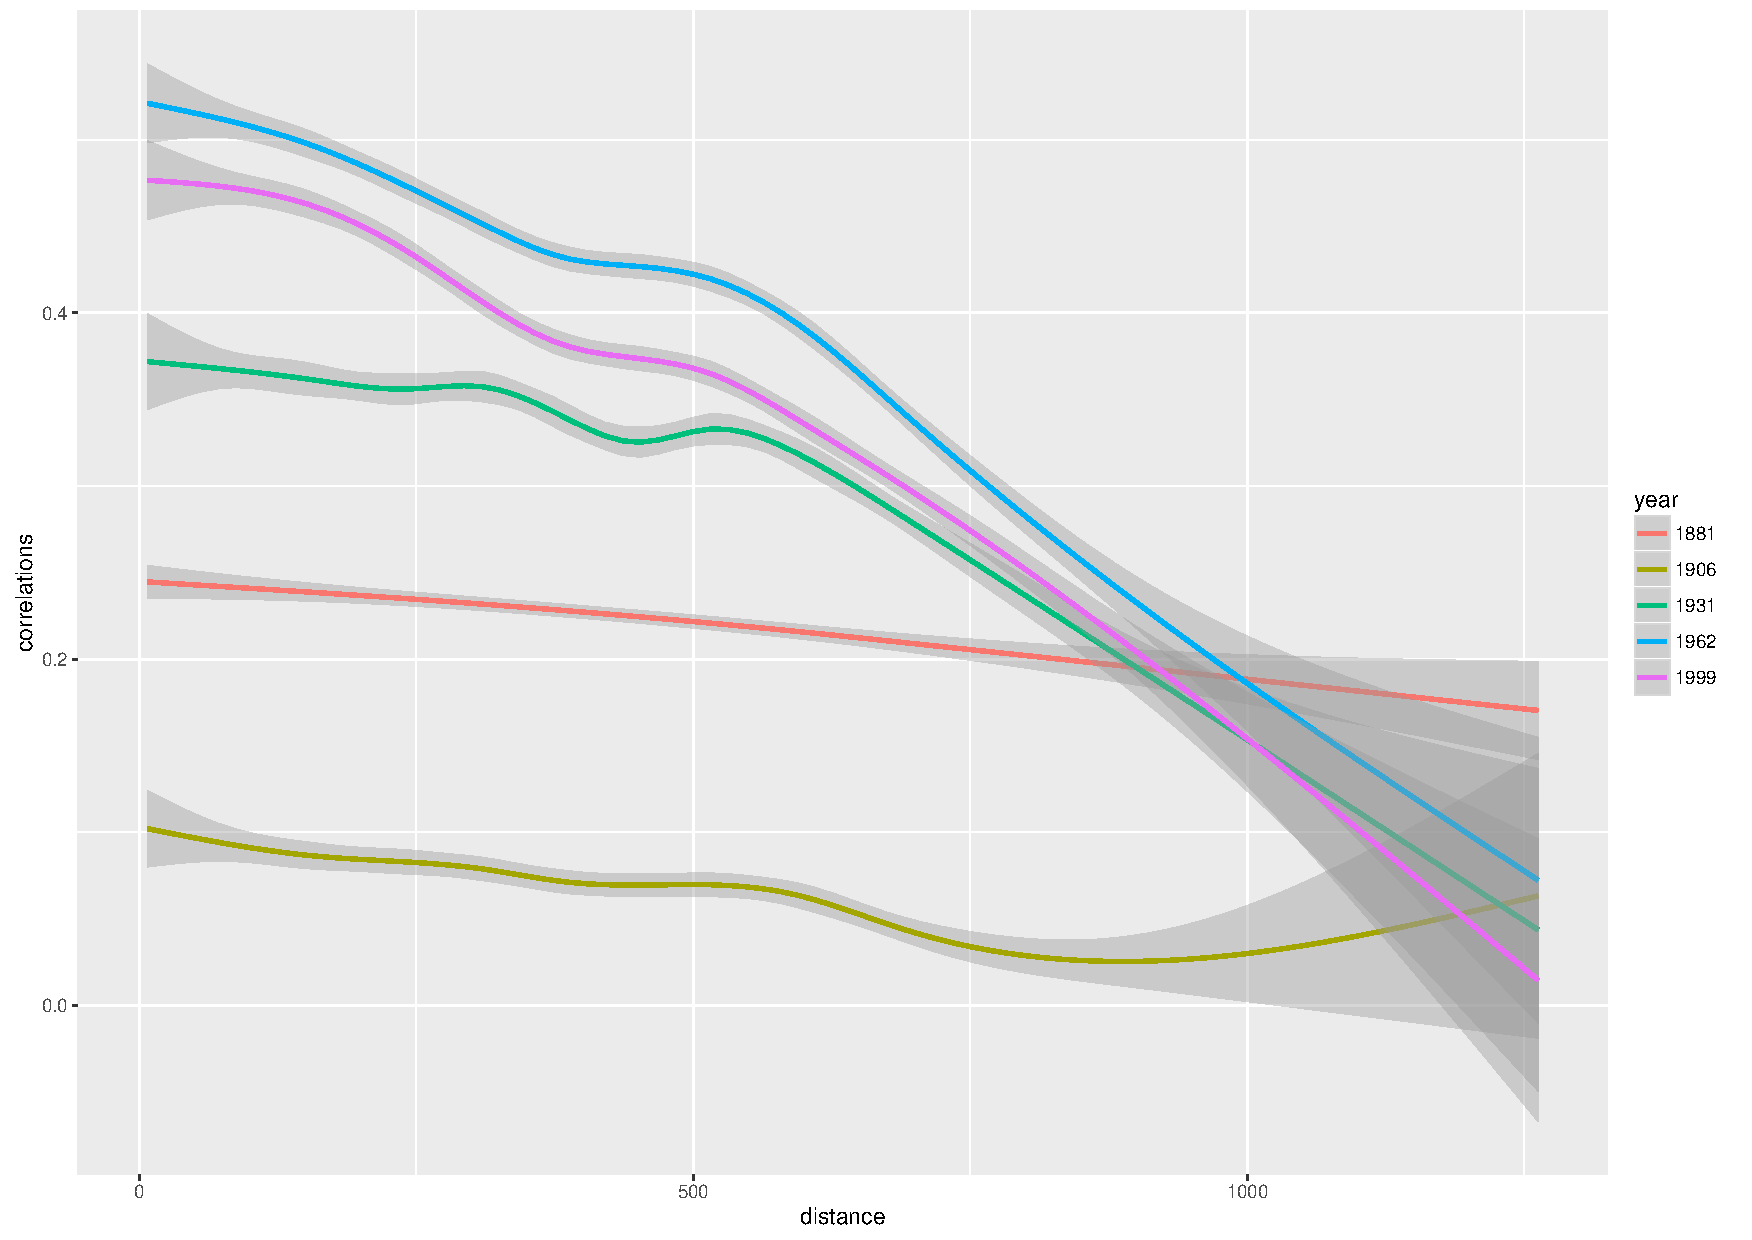
\includegraphics[width=0.6\textwidth]{figures/empirical_tsCorrelations}
}

\sframe{First Modeling Results}{

Interaction model with $\Eb{\vec{P} (t+1)}= (r_0\cdot \mathbf{Id}+\mathbf{R})\Eb{\vec{P}(t)}$, specified with gravity interactions $\left(\mathbf{R}[\cdot]\right)_{ij} = \frac{1}{V_0}\cdot\left(\frac{\Eb{P_j}\Eb{P_i}}{P^2}\right)^{\gamma}\cdot \exp{\left(-\frac{d_ij}{d_0}\right)}$ (note : taking $\gamma=1$ yields linear formulation).

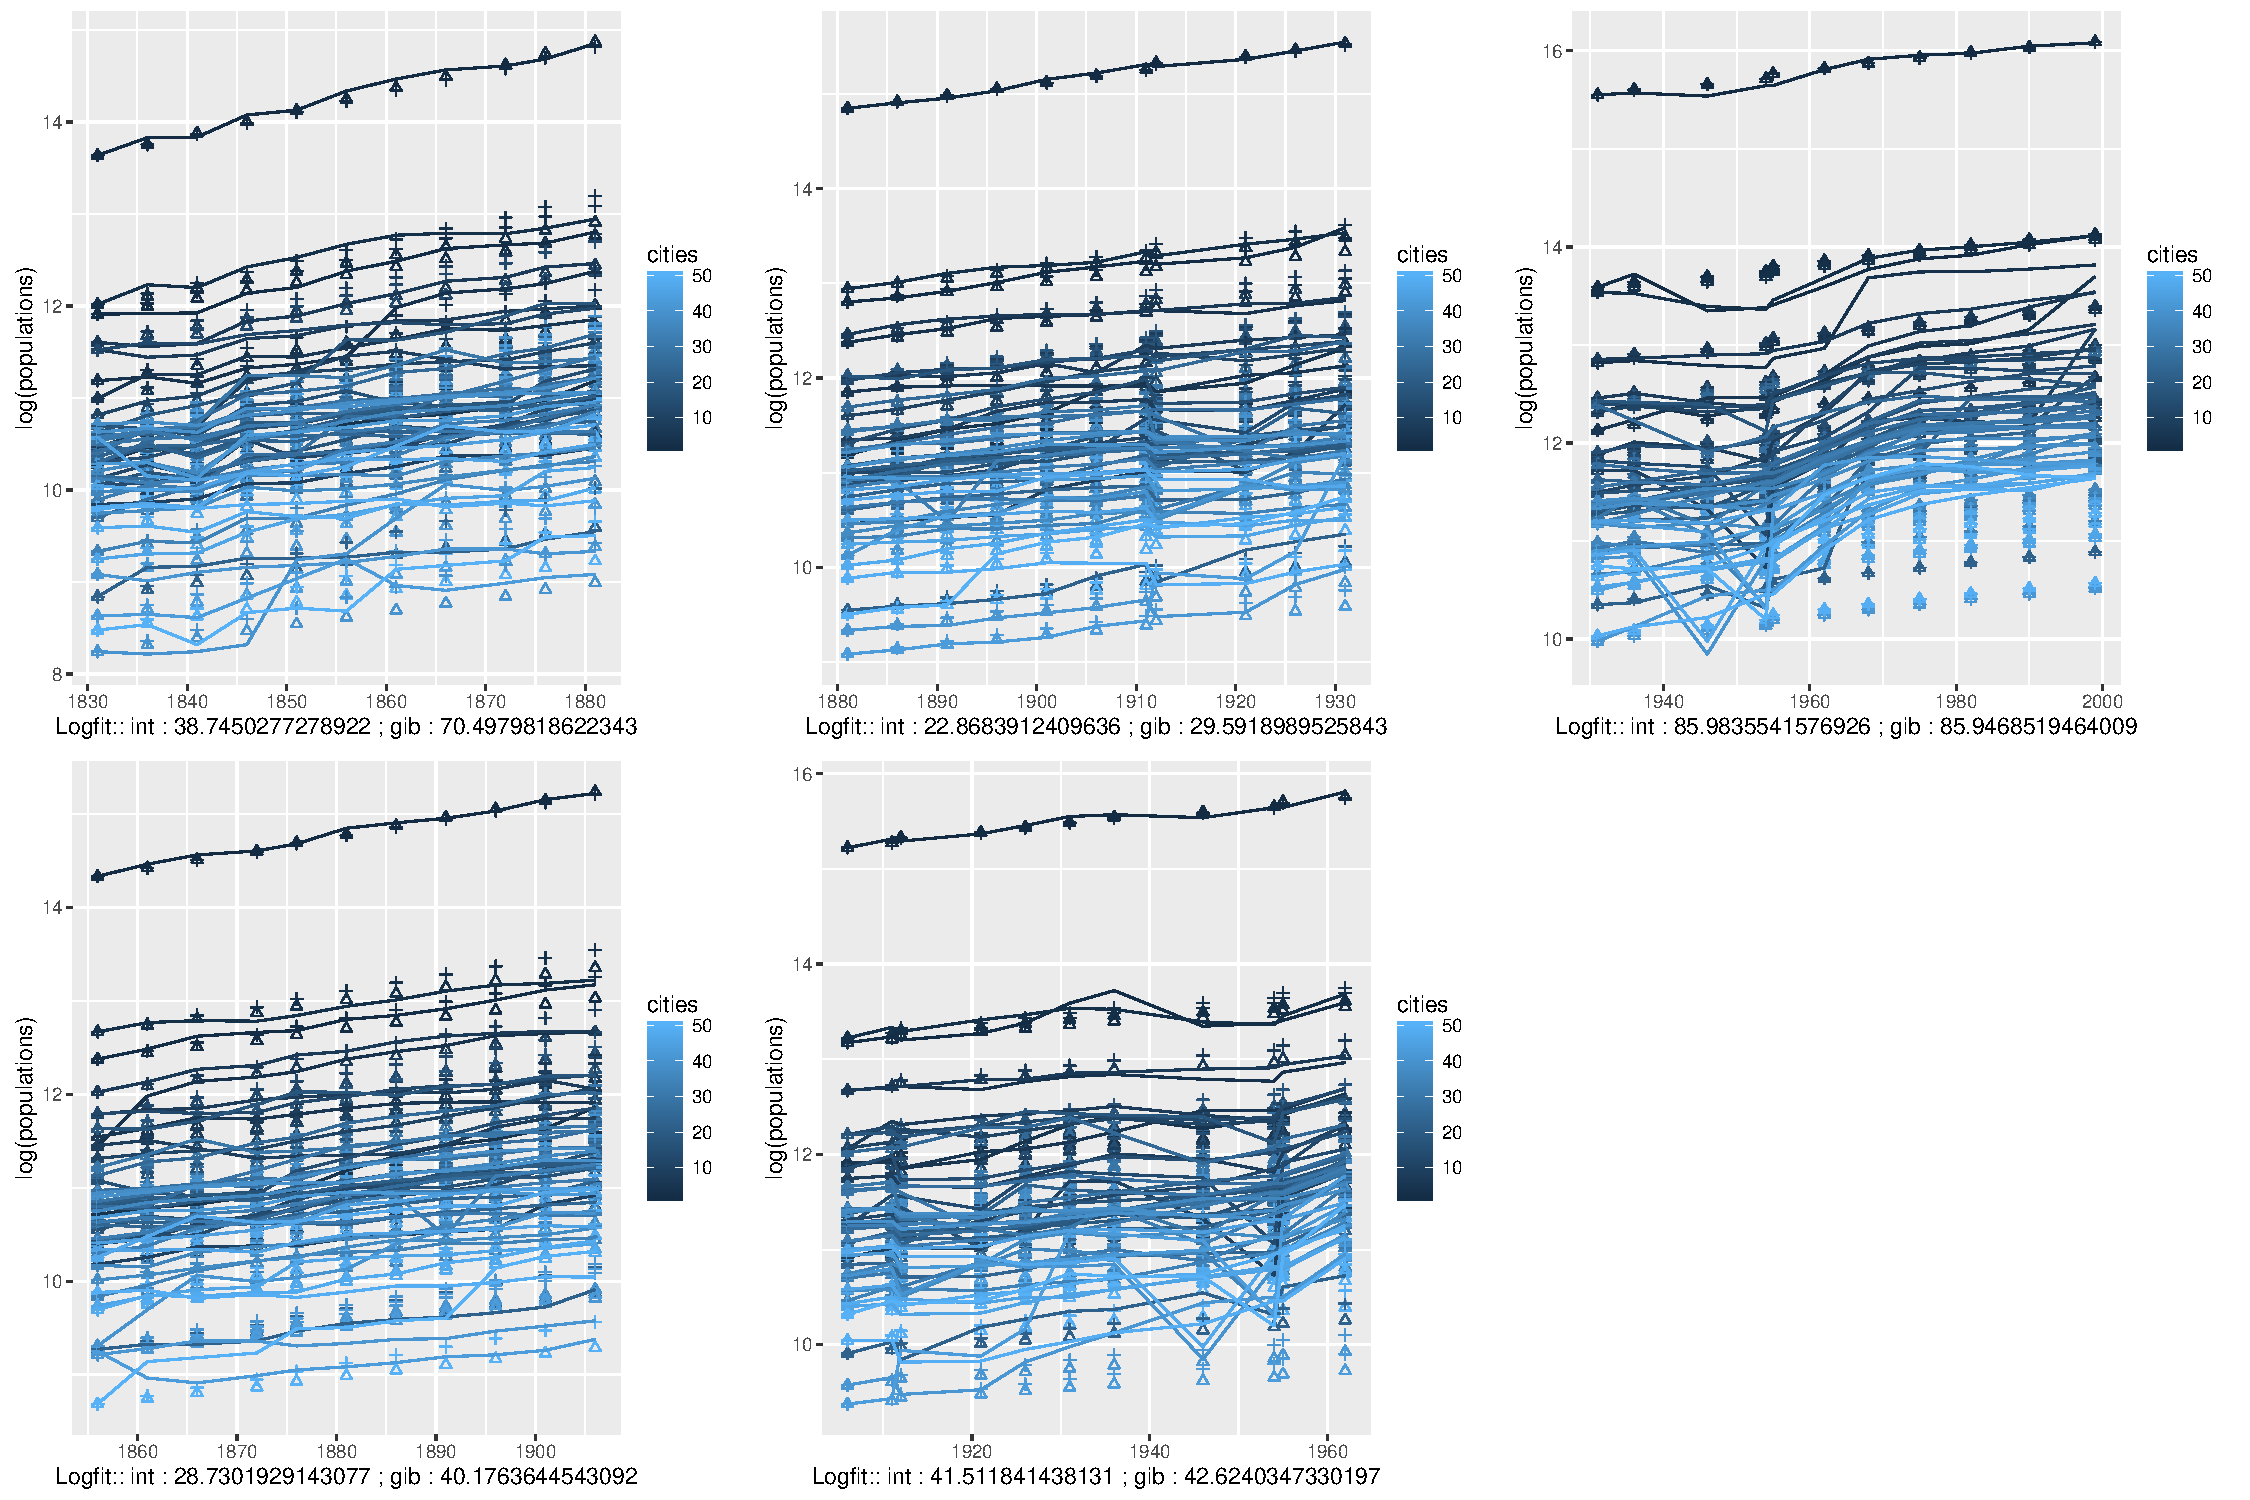
\includegraphics[width=0.8\textwidth]{figures/fit_intgib}
}

\sframe{Methodological Issue}{

\textbf{Next step : } Introduce feedback terms due to effective physical flows passing through the city (in a first approximation only geographically computed with elevation data), test directly for network necessity. Fitting that model should also allow to quantify tunnel effect (strength of feedback).

\bigskip

\textbf{Methodological Flaw : } Issue with overfitting in models of simulations (seems to be an open question) : how do we know fit improvement is not only due to additional degree of freedom ? In stats : AIC provides Kullback-leibler information gain by correcting log-likelihood with number of parameters, nothing similar for models of simulation. Possible solutions :
\small
\begin{enumerate}
\item Empirical version of AIC : Brutal version with empirical likelihood ? Estimation of statistical models on parameter space of each model of simulation, use of corresponding AIC ?
\item Sparse non-linear machine learning to produce a kind of ``absolute'' benchmark explainable variance at a given number or parameters (rq : simple 2nd degree polynomial autoregressive model give far better results than two models above !)
\end{enumerate}


}


\section{China}

\sframe{Terrain in China}{
\textit{5-6 month in China from mid-september, in the frame of Medium project}

Possible specific projects :

\begin{itemize}
\item \textbf{Zhuhai} : in neighborhood of Shenzen/Hong-Kong MCR : particular application of the Lutecia model ; 
\item \textbf{Hangzhou}
\end{itemize}


}



\section{Side Projects}


\sframe{Transportation Equilibrium}{
\textbf{Investigating the Empirical Existence of Static User Equilibrium.}

\textit{3 month of 2-min traffic data for IDF freeways ; explored interactively with shiny app ; spatial and temporal stationarity investigated through spatial and network analysis.}

[accepted (first round) at EWGT 2016]

\medskip

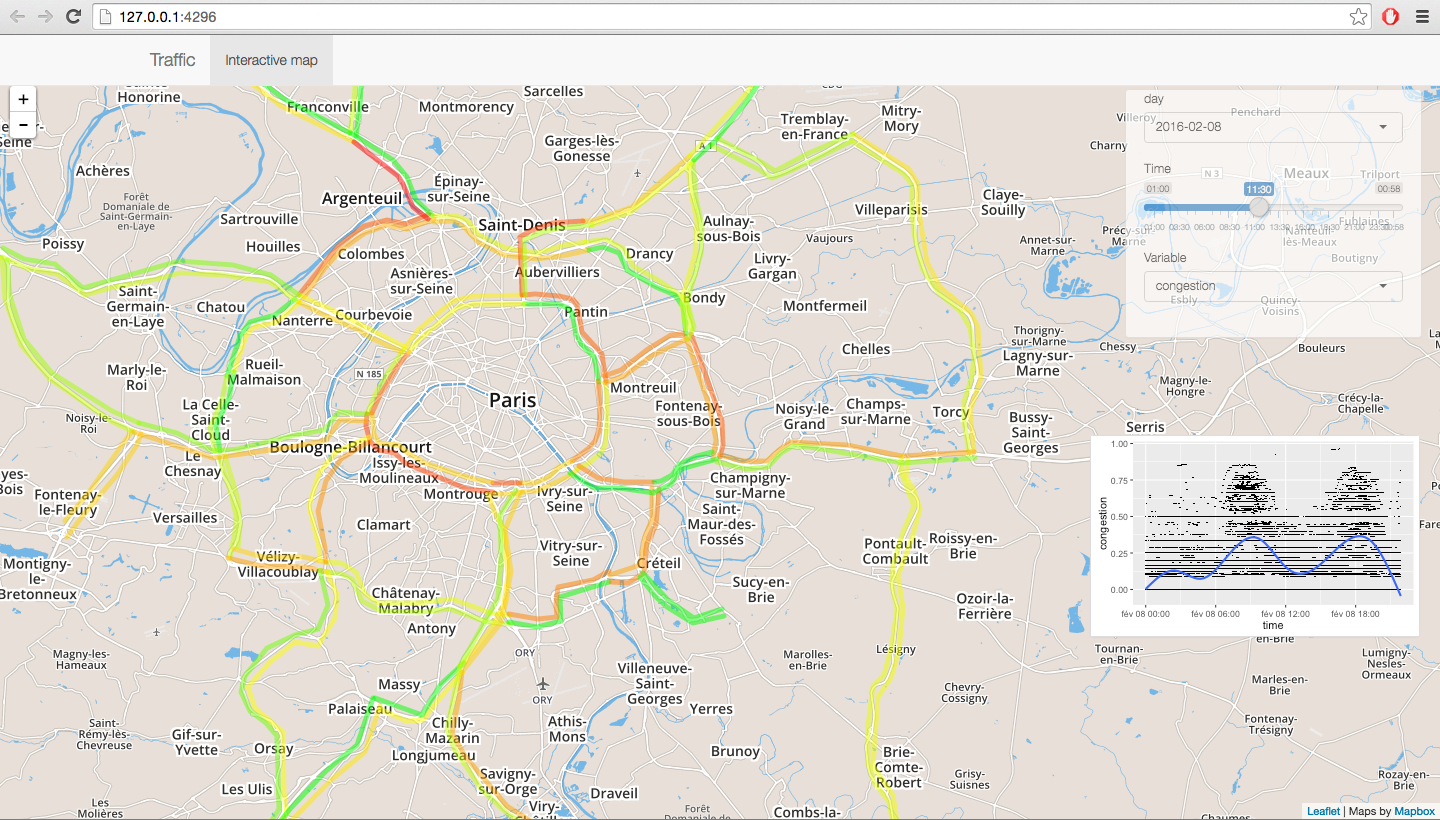
\includegraphics[width=0.35\textwidth]{figures/screen_appli_withplot}
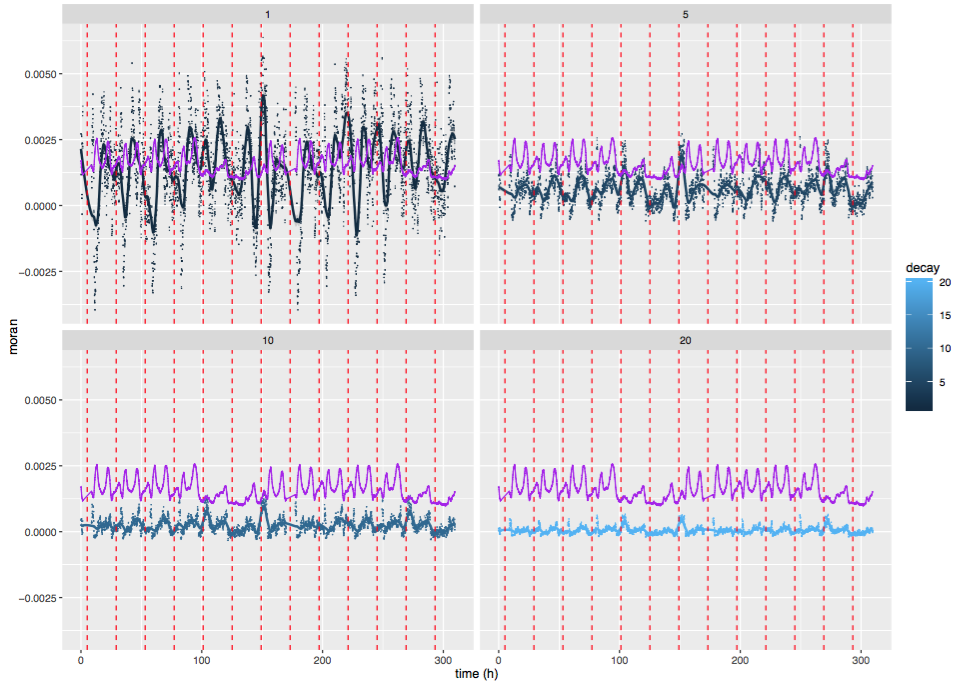
\includegraphics[width=0.35\textwidth]{figures/moran_withCong}
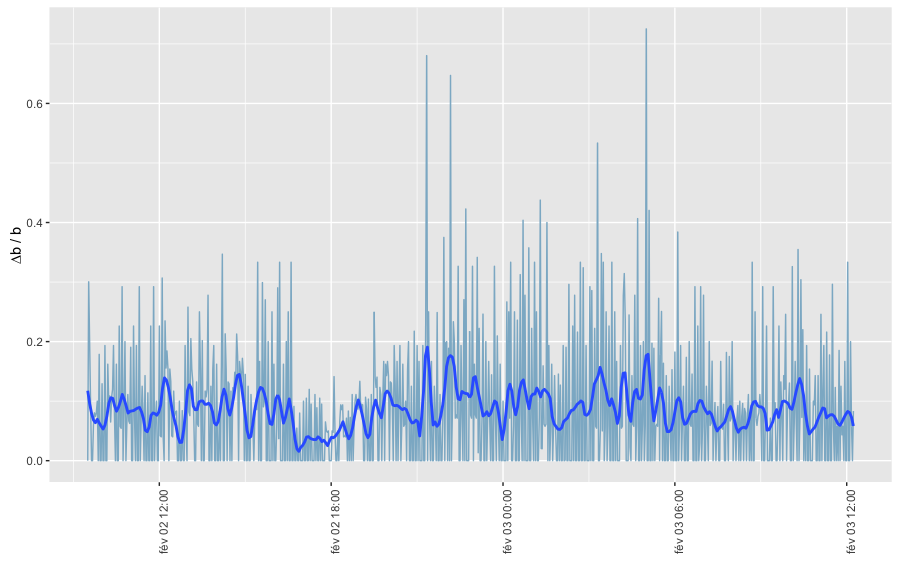
\includegraphics[width=0.35\textwidth]{figures/deltab_sample}
}




\sframe{Discrepancy}{
\textbf{Back on Discrepancy framework for robustness assessment :}\textit{ real geographical application on segregation indicators for metropolitan areas}

[submitted to CSDM 2016]

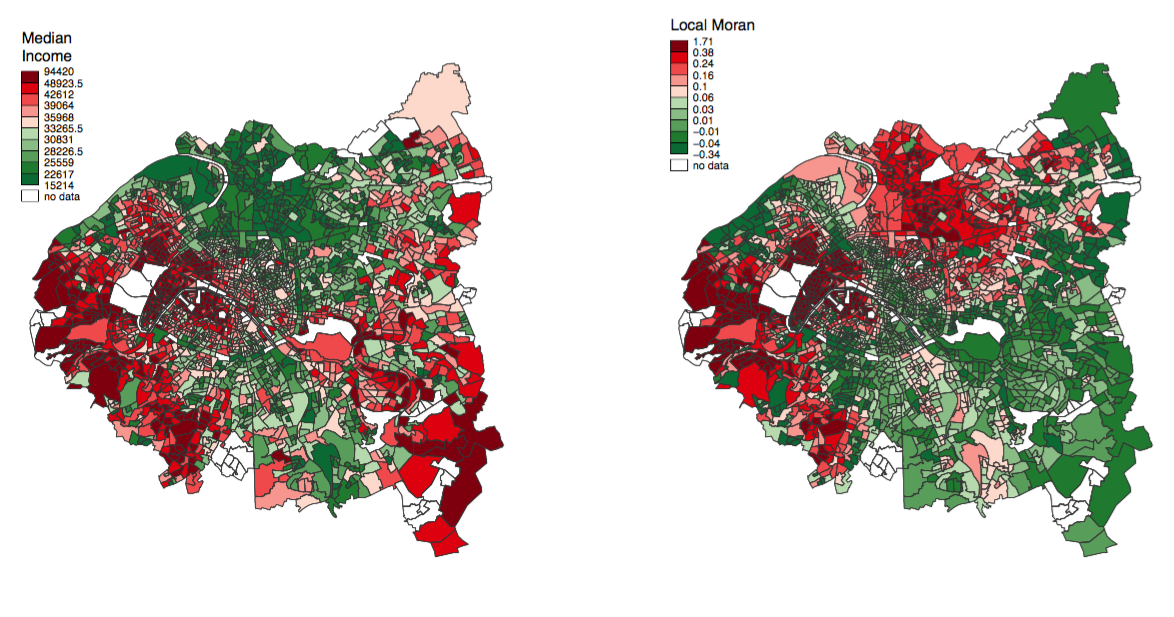
\includegraphics[width=0.55\textwidth]{figures/grandParis_income_moran.png}
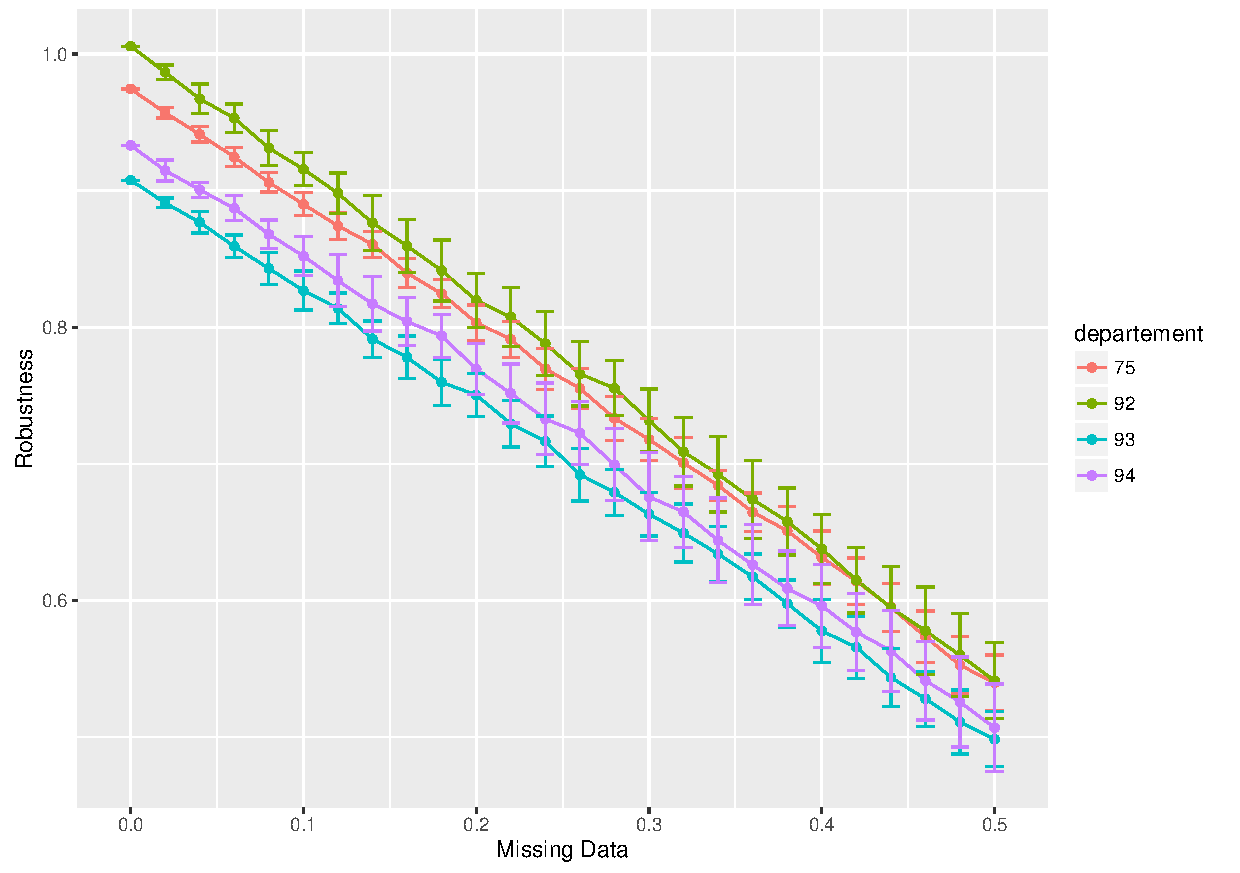
\includegraphics[width=0.55\textwidth]{figures/alldeps_rob}
}


\sframe{Scientific Mediation in Ecology}{
\textbf{Game-based tools as media to transmit freshwater ecology concepts.}

\textit{Agent-based computer game to mediate notions on dynamical stability of ecosystems (prey-predator model) ; complementary with qualitative board-game.}

[poster at SETAC 2016]

\medskip

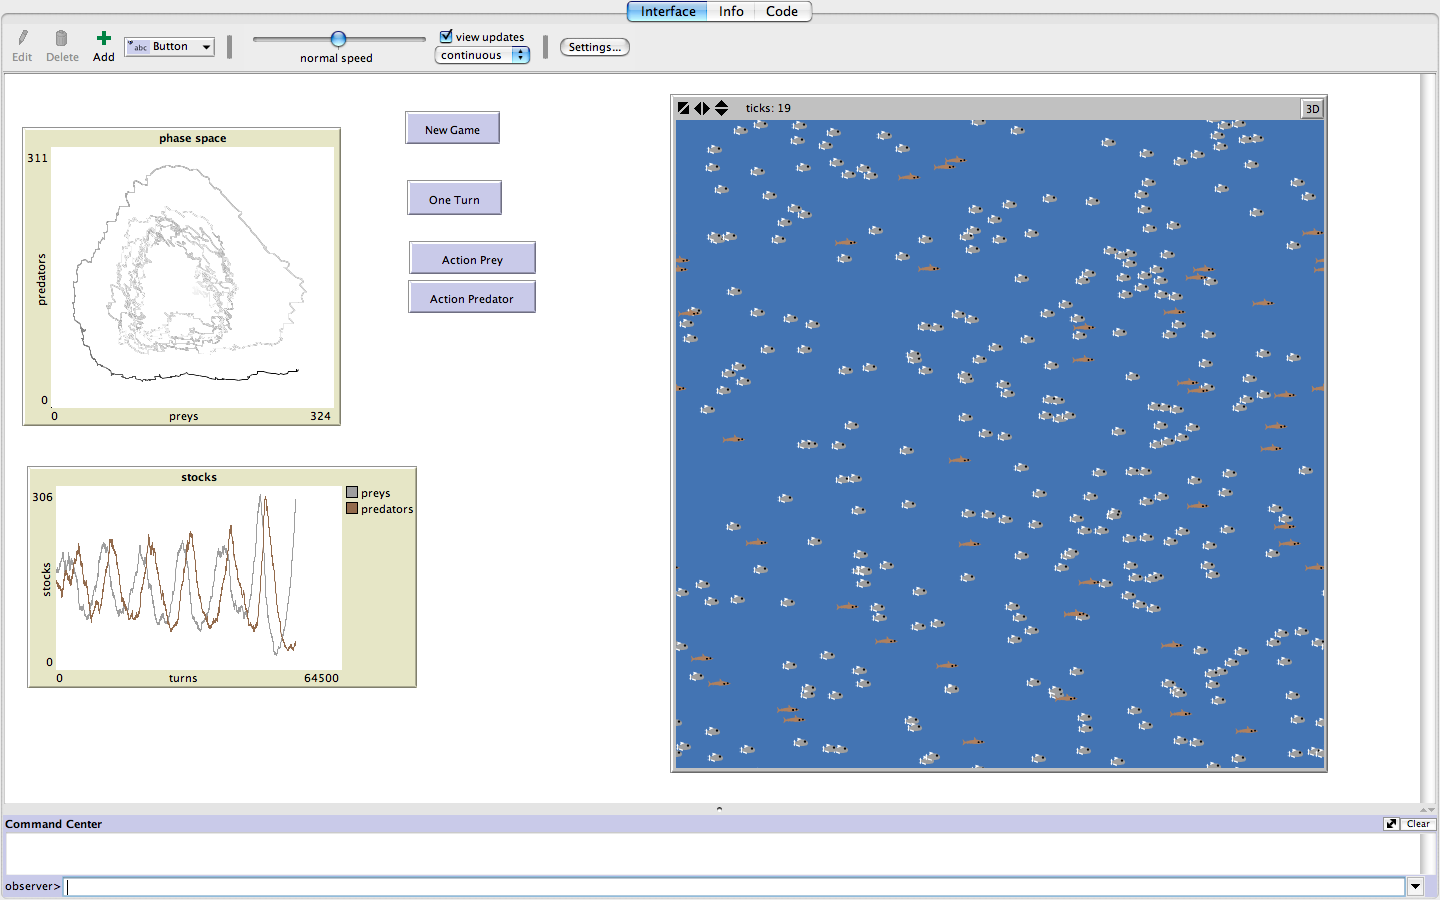
\includegraphics[width=0.55\textwidth]{figures/screen_game}
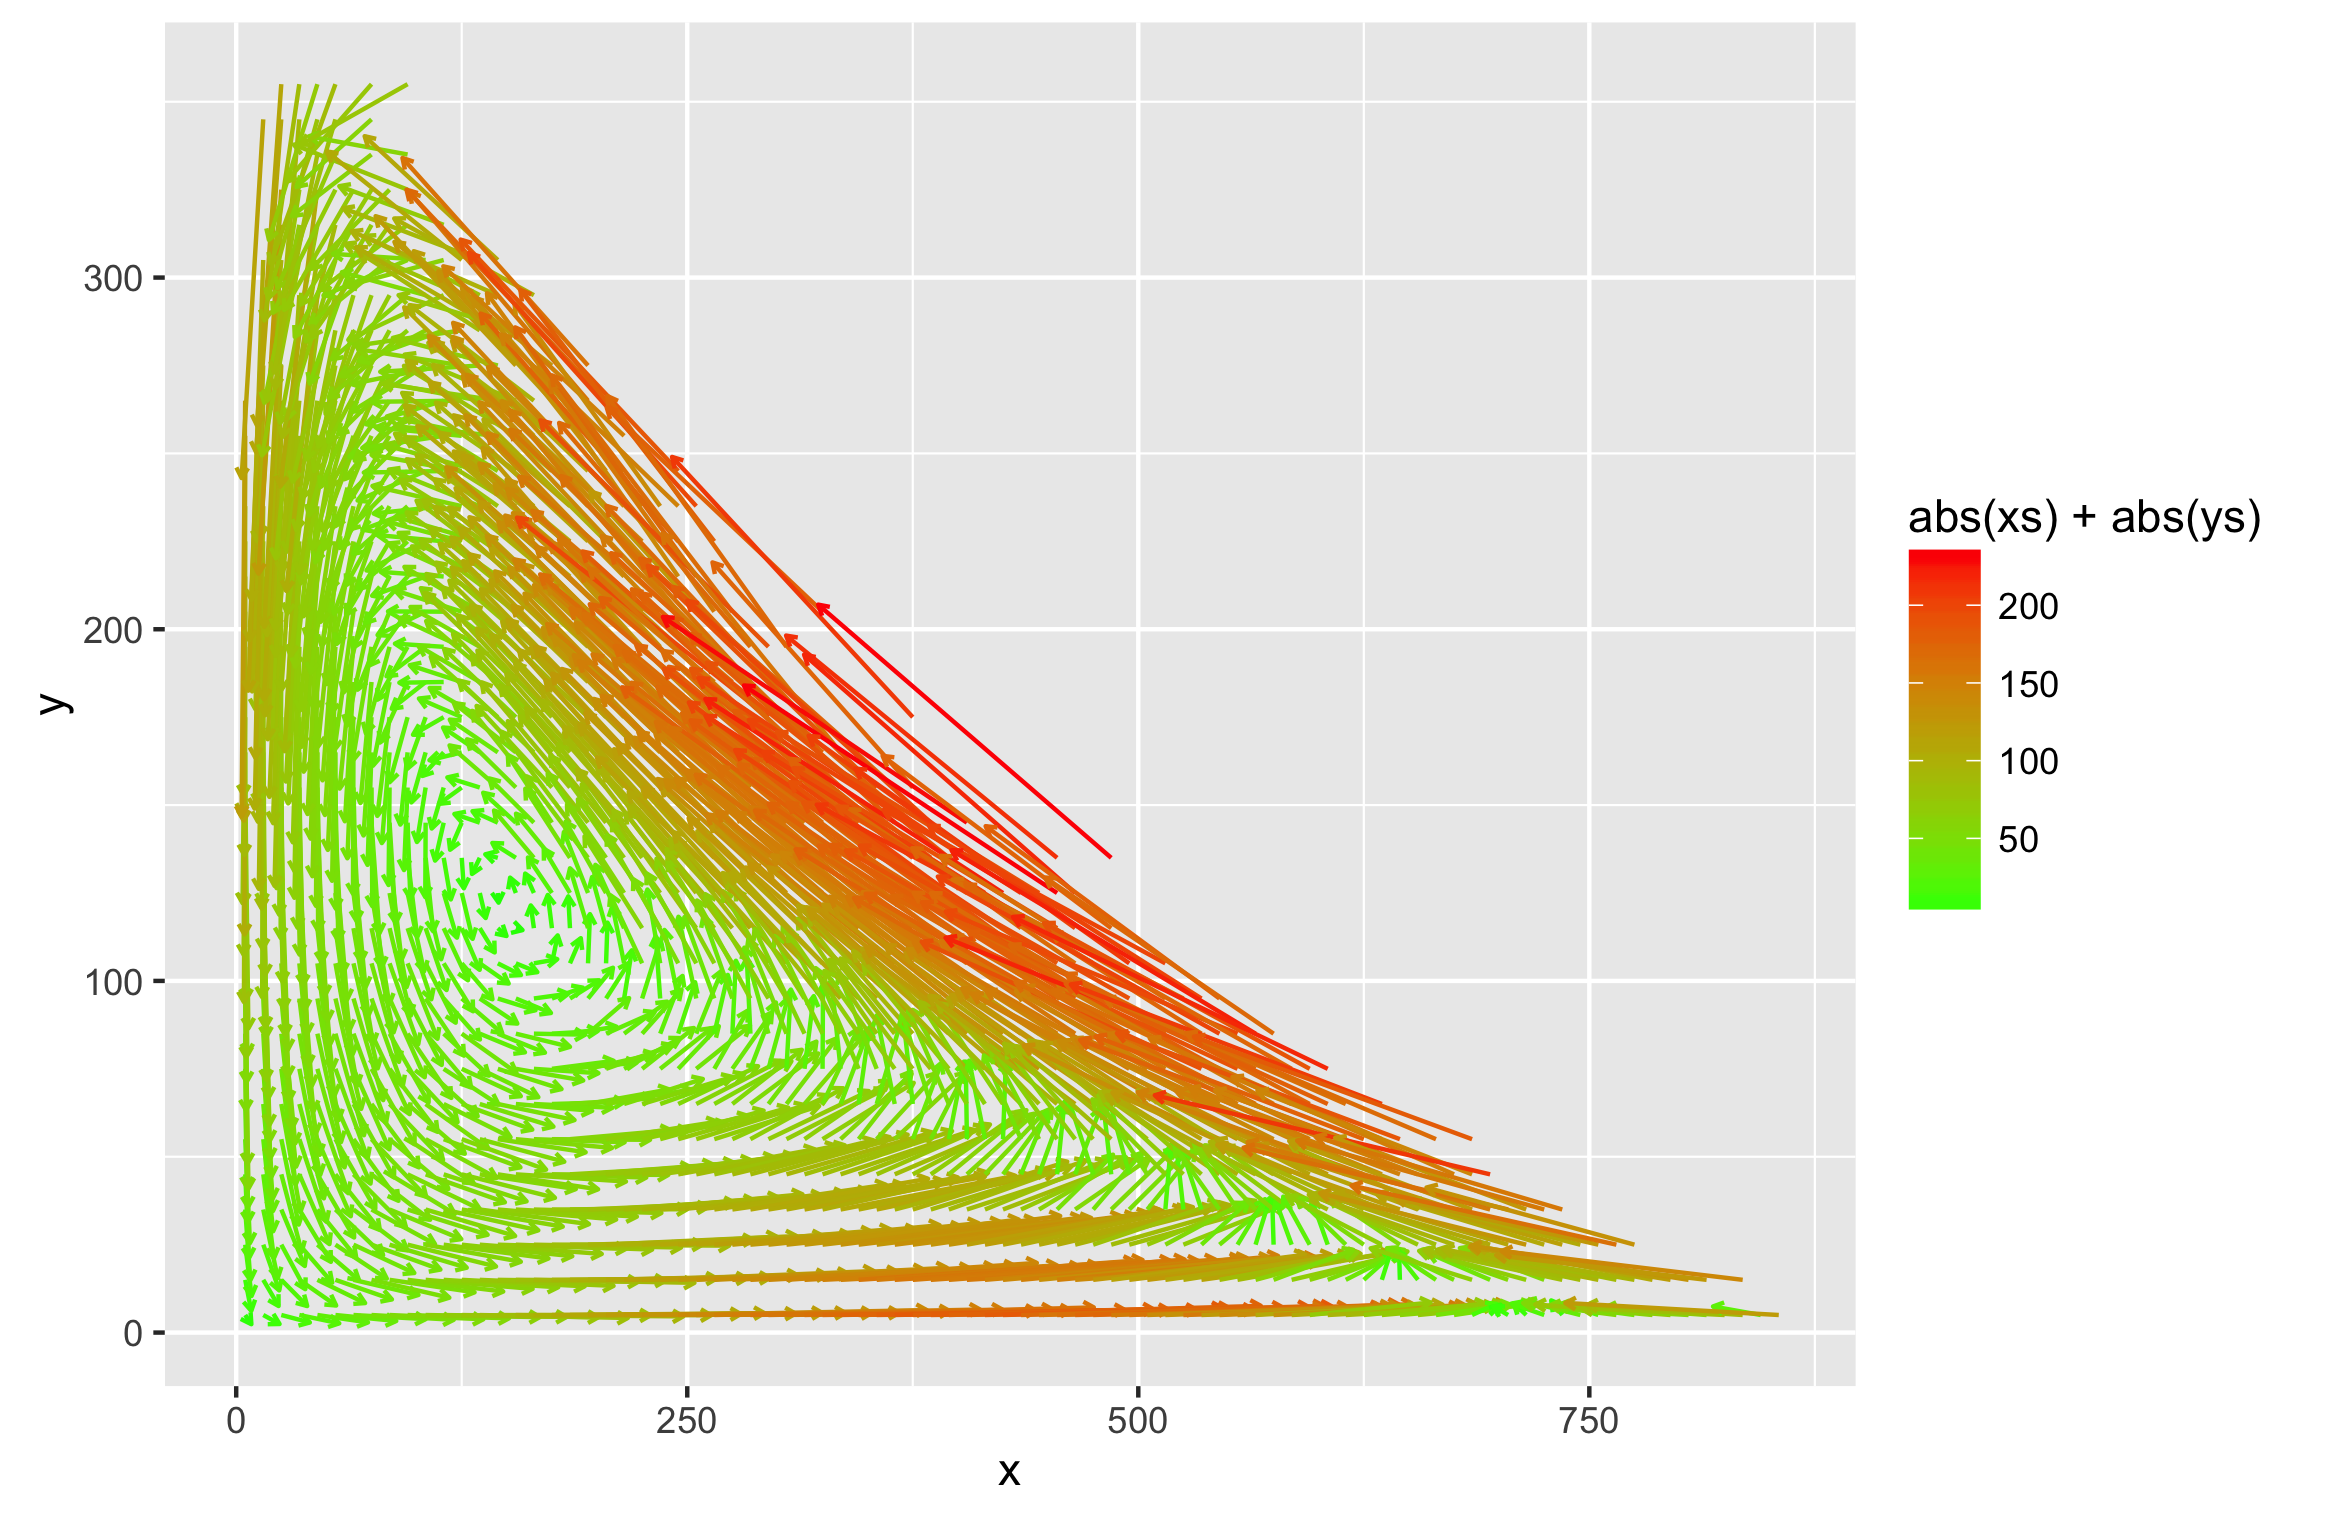
\includegraphics[width=0.55\textwidth]{figures/withGrass1_grassRegrow100_sheepGain20_wolfGain20_sheepRepro5_wolfRepro5}
}





%%%%%%%%%%%%%%%%%%%%%%%%%%%%%%%%
\jframe{Next steps (until June 10th 2016 - SFICSSS departure)}{
\begin{itemize}
\item Theoretical Paper if not crazy ? [1w]\medskip
\item Spatial Statistics / Case studies (Le Corre and Baffi data) [2w]\medskip
\item Cybergeo et al. [1w]\medskip\medskip
\end{itemize}
}






%%%%%%%%%%%%%%%%%%%%%%%%%%%%%%%%
\begin{frame}[allowframebreaks]
\frametitle{References}
\bibliographystyle{apalike}
\bibliography{/Users/Juste/Documents/ComplexSystems/CityNetwork/Biblio/Bibtex/CityNetwork}
\end{frame}
%%%%%%%%%%%%%%%%%%%%%%%%%%%%%%%%


\end{document}




